\documentclass[11pt]{article}

\usepackage{changepage}
\usepackage{graphicx}
\usepackage{amssymb} %math symbols
\usepackage{mathtools} %more math stuff
\usepackage{amsthm} %theorems, proofs and lemmas
\usepackage{optidef} %fast optimization problem notation
\usepackage{biblatex} %Imports biblatex package
\addbibresource{papers.bib} %Import the bibliography file

%% declaring abs so that it works nicely
\DeclarePairedDelimiter\abs{\lvert}{\rvert}%
\DeclarePairedDelimiter\norm{\lVert}{\rVert}%r

\title{MICRO-502 - Aerial Robotics Project}
\author{Filip Slezák, Jean Lesur, Titouan Renard}

\begin{document}

\maketitle

\section{Introduction}

\subsection{Presentation of the Crazyflie platform}

\subsection{Problem statement and discussion of possible pitfalls}

\begin{figure}[h!]
    \centering
    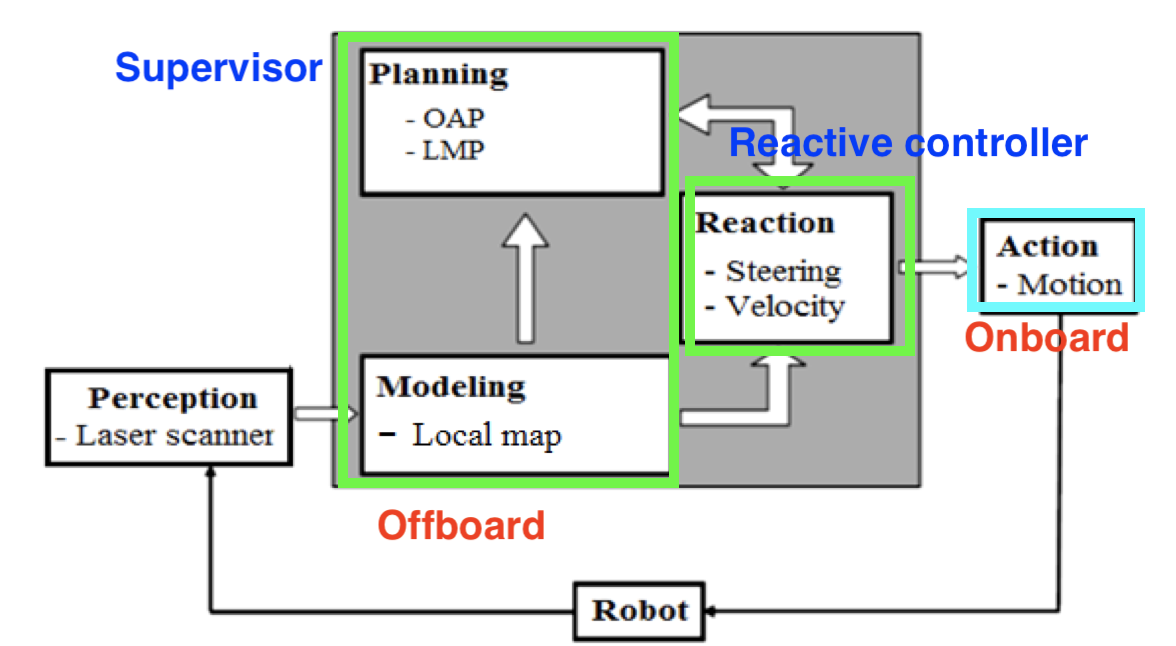
\includegraphics[width=0.5\textwidth]{figures/arch_provisoire.png}
    \caption{Schematic representation of the hybrid architecture.}
    %% Schematic copied from "A hybrid control architecture for autonomous mobile robot navigation in unknown dynamic environment" Nakhaeinia et al. 2015 and modified a bit
\end{figure}


\section{General presentation of our solution}

Our software implements a hybrid-deliberative architecture that can be split into three main components :
\begin{enumerate}
    \item An off-board deliberative \textit{supervisor} that maintains a world model (a map) and ensures the planning of actions
    \item An off-board reactive \textit{controller} that performs navigation tasks (such as take-off, landing and waypoint navigation) while ensuring some guarantees (such as obstacle avoidance)
    \item An on-board control system and state estimator that handles control of the robot
\end{enumerate}


\section{Global navigation and supervisor agent}

In the following section we present the design of the deliberative agent that acts as a

\subsection{Mission-planner finite state machine}

\subsection{Online mapping with uncertainty}

\subsection{Online path planing}

\subsection{Coverage path planning}

\cite{epsilon_star} \cite{Galceran13asurvey} \cite{recsplit}

\tableofcontents

\printbibliography %Prints bibliography

\end{document}
